%% SECTION HEADER /////////////////////////////////////////////////////////////////////////////////////
\section{Model-assisted damage severity assessment}
\label{sec:madif}

%% SECTION CONTENT ////////////////////////////////////////////////////////////////////////////////////

%% SUBSECTION HEADER //////////////////////////////////////////////////////////////////////////////////
The process of determining the damage size is shown in the flowchart in Figure \ref{fig:Flowchart} \cite{fiborek2021model}.
Before inspecting a given \ac{hsc} panel, a numerical analysis has to be performed to determine a function that describes the effect of damage on wave propagation.
Then the model is subjected to experimental validation.
If the simulation results did not agree with the measured results, the material parameters of the components were adjusted.
In the dissertation, the \ac{cfrp} volume fraction of reinforcing fibres was adjusted to determine a wave velocity \cite{kudela2007modelling} and a damping coefficient of the skin to set the magnitude of the registered signals \cite{wandowski2017guided}.
\begin{figure}[!tbh]
	\begin{center}
		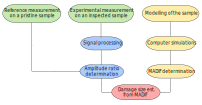
\includegraphics[width=0.95\textwidth]{Chapter_3/flowchart}
	\end{center}
	\caption{A flowchart representing the process for damage size estimation}
	\label{fig:Flowchart}
\end{figure}
\clearpage
When the structure model was developed, several computer simulations for various damage sizes were conducted to determine the \ac{madif}, a cornerstone of the dissertation. This function determines the severity of \ac{hsc} damage based on the signal received by the sensor.
Several excitation signals and damage indices were considered to select the best \ac{madif}.
The selection criterion was the monotonicity and the function slope over the considered range of the damage size. Then, the damage magnitude was obtained from the \ac{madif} for the measured signal and normalised to the reference one.